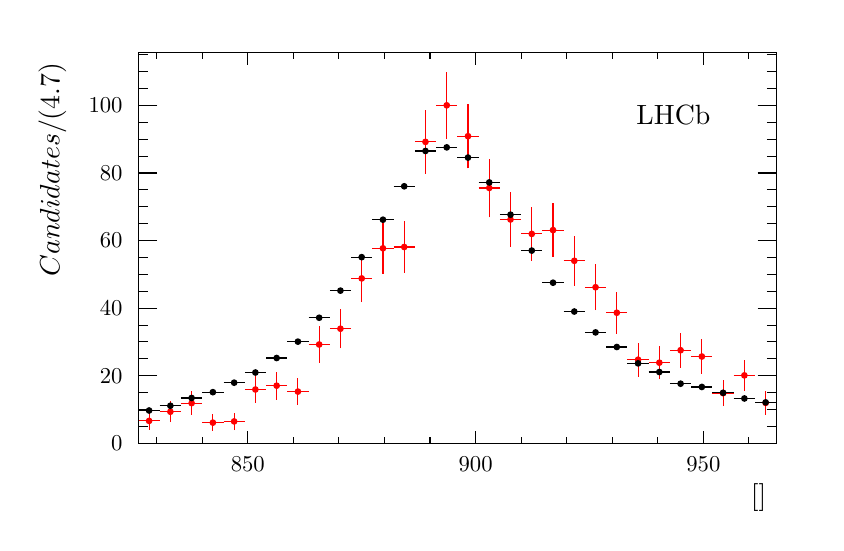
\begin{tikzpicture}
\pgfdeclareplotmark{cross} {
\pgfpathmoveto{\pgfpoint{-0.3\pgfplotmarksize}{\pgfplotmarksize}}
\pgfpathlineto{\pgfpoint{+0.3\pgfplotmarksize}{\pgfplotmarksize}}
\pgfpathlineto{\pgfpoint{+0.3\pgfplotmarksize}{0.3\pgfplotmarksize}}
\pgfpathlineto{\pgfpoint{+1\pgfplotmarksize}{0.3\pgfplotmarksize}}
\pgfpathlineto{\pgfpoint{+1\pgfplotmarksize}{-0.3\pgfplotmarksize}}
\pgfpathlineto{\pgfpoint{+0.3\pgfplotmarksize}{-0.3\pgfplotmarksize}}
\pgfpathlineto{\pgfpoint{+0.3\pgfplotmarksize}{-1.\pgfplotmarksize}}
\pgfpathlineto{\pgfpoint{-0.3\pgfplotmarksize}{-1.\pgfplotmarksize}}
\pgfpathlineto{\pgfpoint{-0.3\pgfplotmarksize}{-0.3\pgfplotmarksize}}
\pgfpathlineto{\pgfpoint{-1.\pgfplotmarksize}{-0.3\pgfplotmarksize}}
\pgfpathlineto{\pgfpoint{-1.\pgfplotmarksize}{0.3\pgfplotmarksize}}
\pgfpathlineto{\pgfpoint{-0.3\pgfplotmarksize}{0.3\pgfplotmarksize}}
\pgfpathclose
\pgfusepathqstroke
}
\pgfdeclareplotmark{cross*} {
\pgfpathmoveto{\pgfpoint{-0.3\pgfplotmarksize}{\pgfplotmarksize}}
\pgfpathlineto{\pgfpoint{+0.3\pgfplotmarksize}{\pgfplotmarksize}}
\pgfpathlineto{\pgfpoint{+0.3\pgfplotmarksize}{0.3\pgfplotmarksize}}
\pgfpathlineto{\pgfpoint{+1\pgfplotmarksize}{0.3\pgfplotmarksize}}
\pgfpathlineto{\pgfpoint{+1\pgfplotmarksize}{-0.3\pgfplotmarksize}}
\pgfpathlineto{\pgfpoint{+0.3\pgfplotmarksize}{-0.3\pgfplotmarksize}}
\pgfpathlineto{\pgfpoint{+0.3\pgfplotmarksize}{-1.\pgfplotmarksize}}
\pgfpathlineto{\pgfpoint{-0.3\pgfplotmarksize}{-1.\pgfplotmarksize}}
\pgfpathlineto{\pgfpoint{-0.3\pgfplotmarksize}{-0.3\pgfplotmarksize}}
\pgfpathlineto{\pgfpoint{-1.\pgfplotmarksize}{-0.3\pgfplotmarksize}}
\pgfpathlineto{\pgfpoint{-1.\pgfplotmarksize}{0.3\pgfplotmarksize}}
\pgfpathlineto{\pgfpoint{-0.3\pgfplotmarksize}{0.3\pgfplotmarksize}}
\pgfpathclose
\pgfusepathqfillstroke
}
\pgfdeclareplotmark{newstar} {
\pgfpathmoveto{\pgfqpoint{0pt}{\pgfplotmarksize}}
\pgfpathlineto{\pgfqpointpolar{44}{0.5\pgfplotmarksize}}
\pgfpathlineto{\pgfqpointpolar{18}{\pgfplotmarksize}}
\pgfpathlineto{\pgfqpointpolar{-20}{0.5\pgfplotmarksize}}
\pgfpathlineto{\pgfqpointpolar{-54}{\pgfplotmarksize}}
\pgfpathlineto{\pgfqpointpolar{-90}{0.5\pgfplotmarksize}}
\pgfpathlineto{\pgfqpointpolar{234}{\pgfplotmarksize}}
\pgfpathlineto{\pgfqpointpolar{198}{0.5\pgfplotmarksize}}
\pgfpathlineto{\pgfqpointpolar{162}{\pgfplotmarksize}}
\pgfpathlineto{\pgfqpointpolar{134}{0.5\pgfplotmarksize}}
\pgfpathclose
\pgfusepathqstroke
}
\pgfdeclareplotmark{newstar*} {
\pgfpathmoveto{\pgfqpoint{0pt}{\pgfplotmarksize}}
\pgfpathlineto{\pgfqpointpolar{44}{0.5\pgfplotmarksize}}
\pgfpathlineto{\pgfqpointpolar{18}{\pgfplotmarksize}}
\pgfpathlineto{\pgfqpointpolar{-20}{0.5\pgfplotmarksize}}
\pgfpathlineto{\pgfqpointpolar{-54}{\pgfplotmarksize}}
\pgfpathlineto{\pgfqpointpolar{-90}{0.5\pgfplotmarksize}}
\pgfpathlineto{\pgfqpointpolar{234}{\pgfplotmarksize}}
\pgfpathlineto{\pgfqpointpolar{198}{0.5\pgfplotmarksize}}
\pgfpathlineto{\pgfqpointpolar{162}{\pgfplotmarksize}}
\pgfpathlineto{\pgfqpointpolar{134}{0.5\pgfplotmarksize}}
\pgfpathclose
\pgfusepathqfillstroke
}
\definecolor{c}{rgb}{1,1,1};
\draw [color=c, fill=c] (0,0) rectangle (10,6.27517);
\draw [color=c, fill=c] (1.4,1.00403) rectangle (9.5,5.96141);
\definecolor{c}{rgb}{0,0,0};
\draw [c] (1.4,1.00403) -- (1.4,5.96141) -- (9.5,5.96141) -- (9.5,1.00403) -- (1.4,1.00403);
\definecolor{c}{rgb}{1,1,1};
\draw [color=c, fill=c] (1.4,1.00403) rectangle (9.5,5.96141);
\definecolor{c}{rgb}{0,0,0};
\draw [c] (1.4,1.00403) -- (1.4,5.96141) -- (9.5,5.96141) -- (9.5,1.00403) -- (1.4,1.00403);
\definecolor{c}{rgb}{1,0,0};
\draw [c,line width=0.4] (1.535,1.17784) -- (1.535,1.28827);
\draw [c,line width=0.4] (1.535,1.28827) -- (1.535,1.39869);
\draw [c,line width=0.4] (1.4,1.28827) -- (1.535,1.28827);
\draw [c,line width=0.4] (1.535,1.28827) -- (1.67,1.28827);
\foreach \P in {(1.535,1.28827)}{\draw[mark options={color=c,fill=c},mark size=2.402402pt,mark=*,mark size=1pt] plot coordinates {\P};}
\draw [c,line width=0.4] (1.805,1.27348) -- (1.805,1.40456);
\draw [c,line width=0.4] (1.805,1.40456) -- (1.805,1.53565);
\draw [c,line width=0.4] (1.67,1.40456) -- (1.805,1.40456);
\draw [c,line width=0.4] (1.805,1.40456) -- (1.94,1.40456);
\foreach \P in {(1.805,1.40456)}{\draw[mark options={color=c,fill=c},mark size=2.402402pt,mark=*,mark size=1pt] plot coordinates {\P};}
\draw [c,line width=0.4] (2.075,1.36594) -- (2.075,1.51382);
\draw [c,line width=0.4] (2.075,1.51382) -- (2.075,1.6617);
\draw [c,line width=0.4] (1.94,1.51382) -- (2.075,1.51382);
\draw [c,line width=0.4] (2.075,1.51382) -- (2.21,1.51382);
\foreach \P in {(2.075,1.51382)}{\draw[mark options={color=c,fill=c},mark size=2.402402pt,mark=*,mark size=1pt] plot coordinates {\P};}
\draw [c,line width=0.4] (2.345,1.16002) -- (2.345,1.26604);
\draw [c,line width=0.4] (2.345,1.26604) -- (2.345,1.37205);
\draw [c,line width=0.4] (2.21,1.26604) -- (2.345,1.26604);
\draw [c,line width=0.4] (2.345,1.26604) -- (2.48,1.26604);
\foreach \P in {(2.345,1.26604)}{\draw[mark options={color=c,fill=c},mark size=2.402402pt,mark=*,mark size=1pt] plot coordinates {\P};}
\draw [c,line width=0.4] (2.615,1.17259) -- (2.615,1.28174);
\draw [c,line width=0.4] (2.615,1.28174) -- (2.615,1.39089);
\draw [c,line width=0.4] (2.48,1.28174) -- (2.615,1.28174);
\draw [c,line width=0.4] (2.615,1.28174) -- (2.75,1.28174);
\foreach \P in {(2.615,1.28174)}{\draw[mark options={color=c,fill=c},mark size=2.402402pt,mark=*,mark size=1pt] plot coordinates {\P};}
\draw [c,line width=0.4] (2.885,1.51579) -- (2.885,1.68695);
\draw [c,line width=0.4] (2.885,1.68695) -- (2.885,1.85811);
\draw [c,line width=0.4] (2.75,1.68695) -- (2.885,1.68695);
\draw [c,line width=0.4] (2.885,1.68695) -- (3.02,1.68695);
\foreach \P in {(2.885,1.68695)}{\draw[mark options={color=c,fill=c},mark size=2.402402pt,mark=*,mark size=1pt] plot coordinates {\P};}
\draw [c,line width=0.4] (3.155,1.55856) -- (3.155,1.73572);
\draw [c,line width=0.4] (3.155,1.73572) -- (3.155,1.91289);
\draw [c,line width=0.4] (3.02,1.73572) -- (3.155,1.73572);
\draw [c,line width=0.4] (3.155,1.73572) -- (3.29,1.73572);
\foreach \P in {(3.155,1.73572)}{\draw[mark options={color=c,fill=c},mark size=2.402402pt,mark=*,mark size=1pt] plot coordinates {\P};}
\draw [c,line width=0.4] (3.425,1.49251) -- (3.425,1.6603);
\draw [c,line width=0.4] (3.425,1.6603) -- (3.425,1.82808);
\draw [c,line width=0.4] (3.29,1.6603) -- (3.425,1.6603);
\draw [c,line width=0.4] (3.425,1.6603) -- (3.56,1.6603);
\foreach \P in {(3.425,1.6603)}{\draw[mark options={color=c,fill=c},mark size=2.402402pt,mark=*,mark size=1pt] plot coordinates {\P};}
\draw [c,line width=0.4] (3.695,2.02663) -- (3.695,2.25862);
\draw [c,line width=0.4] (3.695,2.25862) -- (3.695,2.49061);
\draw [c,line width=0.4] (3.56,2.25862) -- (3.695,2.25862);
\draw [c,line width=0.4] (3.695,2.25862) -- (3.83,2.25862);
\foreach \P in {(3.695,2.25862)}{\draw[mark options={color=c,fill=c},mark size=2.402402pt,mark=*,mark size=1pt] plot coordinates {\P};}
\draw [c,line width=0.4] (3.965,2.209) -- (3.965,2.45881);
\draw [c,line width=0.4] (3.965,2.45881) -- (3.965,2.70862);
\draw [c,line width=0.4] (3.83,2.45881) -- (3.965,2.45881);
\draw [c,line width=0.4] (3.965,2.45881) -- (4.1,2.45881);
\foreach \P in {(3.965,2.45881)}{\draw[mark options={color=c,fill=c},mark size=2.402402pt,mark=*,mark size=1pt] plot coordinates {\P};}
\draw [c,line width=0.4] (4.235,2.79809) -- (4.235,3.09778);
\draw [c,line width=0.4] (4.235,3.09778) -- (4.235,3.39748);
\draw [c,line width=0.4] (4.1,3.09778) -- (4.235,3.09778);
\draw [c,line width=0.4] (4.235,3.09778) -- (4.37,3.09778);
\foreach \P in {(4.235,3.09778)}{\draw[mark options={color=c,fill=c},mark size=2.402402pt,mark=*,mark size=1pt] plot coordinates {\P};}
\draw [c,line width=0.4] (4.505,3.1545) -- (4.505,3.48044);
\draw [c,line width=0.4] (4.505,3.48044) -- (4.505,3.80637);
\draw [c,line width=0.4] (4.37,3.48044) -- (4.505,3.48044);
\draw [c,line width=0.4] (4.505,3.48044) -- (4.64,3.48044);
\foreach \P in {(4.505,3.48044)}{\draw[mark options={color=c,fill=c},mark size=2.402402pt,mark=*,mark size=1pt] plot coordinates {\P};}
\draw [c,line width=0.4] (4.775,3.16967) -- (4.775,3.49667);
\draw [c,line width=0.4] (4.775,3.49667) -- (4.775,3.82366);
\draw [c,line width=0.4] (4.64,3.49667) -- (4.775,3.49667);
\draw [c,line width=0.4] (4.775,3.49667) -- (4.91,3.49667);
\foreach \P in {(4.775,3.49667)}{\draw[mark options={color=c,fill=c},mark size=2.402402pt,mark=*,mark size=1pt] plot coordinates {\P};}
\draw [c,line width=0.4] (5.045,4.42665) -- (5.045,4.83187);
\draw [c,line width=0.4] (5.045,4.83187) -- (5.045,5.23709);
\draw [c,line width=0.4] (4.91,4.83187) -- (5.045,4.83187);
\draw [c,line width=0.4] (5.045,4.83187) -- (5.18,4.83187);
\foreach \P in {(5.045,4.83187)}{\draw[mark options={color=c,fill=c},mark size=2.402402pt,mark=*,mark size=1pt] plot coordinates {\P};}
\draw [c,line width=0.4] (5.315,4.86715) -- (5.315,5.29625);
\draw [c,line width=0.4] (5.315,5.29625) -- (5.315,5.72534);
\draw [c,line width=0.4] (5.18,5.29625) -- (5.315,5.29625);
\draw [c,line width=0.4] (5.315,5.29625) -- (5.45,5.29625);
\foreach \P in {(5.315,5.29625)}{\draw[mark options={color=c,fill=c},mark size=2.402402pt,mark=*,mark size=1pt] plot coordinates {\P};}
\draw [c,line width=0.4] (5.585,4.4952) -- (5.585,4.90423);
\draw [c,line width=0.4] (5.585,4.90423) -- (5.585,5.31327);
\draw [c,line width=0.4] (5.45,4.90423) -- (5.585,4.90423);
\draw [c,line width=0.4] (5.585,4.90423) -- (5.72,4.90423);
\foreach \P in {(5.585,4.90423)}{\draw[mark options={color=c,fill=c},mark size=2.402402pt,mark=*,mark size=1pt] plot coordinates {\P};}
\draw [c,line width=0.4] (5.855,3.87371) -- (5.855,4.24667);
\draw [c,line width=0.4] (5.855,4.24667) -- (5.855,4.61964);
\draw [c,line width=0.4] (5.72,4.24667) -- (5.855,4.24667);
\draw [c,line width=0.4] (5.855,4.24667) -- (5.99,4.24667);
\foreach \P in {(5.855,4.24667)}{\draw[mark options={color=c,fill=c},mark size=2.402402pt,mark=*,mark size=1pt] plot coordinates {\P};}
\draw [c,line width=0.4] (6.125,3.49716) -- (6.125,3.84635);
\draw [c,line width=0.4] (6.125,3.84635) -- (6.125,4.19553);
\draw [c,line width=0.4] (5.99,3.84635) -- (6.125,3.84635);
\draw [c,line width=0.4] (6.125,3.84635) -- (6.26,3.84635);
\foreach \P in {(6.125,3.84635)}{\draw[mark options={color=c,fill=c},mark size=2.402402pt,mark=*,mark size=1pt] plot coordinates {\P};}
\draw [c,line width=0.4] (6.395,3.32518) -- (6.395,3.66291);
\draw [c,line width=0.4] (6.395,3.66291) -- (6.395,4.00064);
\draw [c,line width=0.4] (6.26,3.66291) -- (6.395,3.66291);
\draw [c,line width=0.4] (6.395,3.66291) -- (6.53,3.66291);
\foreach \P in {(6.395,3.66291)}{\draw[mark options={color=c,fill=c},mark size=2.402402pt,mark=*,mark size=1pt] plot coordinates {\P};}
\draw [c,line width=0.4] (6.665,3.37055) -- (6.665,3.71134);
\draw [c,line width=0.4] (6.665,3.71134) -- (6.665,4.05213);
\draw [c,line width=0.4] (6.53,3.71134) -- (6.665,3.71134);
\draw [c,line width=0.4] (6.665,3.71134) -- (6.8,3.71134);
\foreach \P in {(6.665,3.71134)}{\draw[mark options={color=c,fill=c},mark size=2.402402pt,mark=*,mark size=1pt] plot coordinates {\P};}
\draw [c,line width=0.4] (6.935,3.00614) -- (6.935,3.32143);
\draw [c,line width=0.4] (6.935,3.32143) -- (6.935,3.63673);
\draw [c,line width=0.4] (6.8,3.32143) -- (6.935,3.32143);
\draw [c,line width=0.4] (6.935,3.32143) -- (7.07,3.32143);
\foreach \P in {(6.935,3.32143)}{\draw[mark options={color=c,fill=c},mark size=2.402402pt,mark=*,mark size=1pt] plot coordinates {\P};}
\draw [c,line width=0.4] (7.205,2.69423) -- (7.205,2.9858);
\draw [c,line width=0.4] (7.205,2.9858) -- (7.205,3.27737);
\draw [c,line width=0.4] (7.07,2.9858) -- (7.205,2.9858);
\draw [c,line width=0.4] (7.205,2.9858) -- (7.34,2.9858);
\foreach \P in {(7.205,2.9858)}{\draw[mark options={color=c,fill=c},mark size=2.402402pt,mark=*,mark size=1pt] plot coordinates {\P};}
\draw [c,line width=0.4] (7.475,2.39511) -- (7.475,2.66178);
\draw [c,line width=0.4] (7.475,2.66178) -- (7.475,2.92845);
\draw [c,line width=0.4] (7.34,2.66178) -- (7.475,2.66178);
\draw [c,line width=0.4] (7.475,2.66178) -- (7.61,2.66178);
\foreach \P in {(7.475,2.66178)}{\draw[mark options={color=c,fill=c},mark size=2.402402pt,mark=*,mark size=1pt] plot coordinates {\P};}
\draw [c,line width=0.4] (7.745,1.85202) -- (7.745,2.0654);
\draw [c,line width=0.4] (7.745,2.0654) -- (7.745,2.27878);
\draw [c,line width=0.4] (7.61,2.0654) -- (7.745,2.0654);
\draw [c,line width=0.4] (7.745,2.0654) -- (7.88,2.0654);
\foreach \P in {(7.745,2.0654)}{\draw[mark options={color=c,fill=c},mark size=2.402402pt,mark=*,mark size=1pt] plot coordinates {\P};}
\draw [c,line width=0.4] (8.015,1.81816) -- (8.015,2.02772);
\draw [c,line width=0.4] (8.015,2.02772) -- (8.015,2.23728);
\draw [c,line width=0.4] (7.88,2.02772) -- (8.015,2.02772);
\draw [c,line width=0.4] (8.015,2.02772) -- (8.15,2.02772);
\foreach \P in {(8.015,2.02772)}{\draw[mark options={color=c,fill=c},mark size=2.402402pt,mark=*,mark size=1pt] plot coordinates {\P};}
\draw [c,line width=0.4] (8.285,1.96043) -- (8.285,2.18556);
\draw [c,line width=0.4] (8.285,2.18556) -- (8.285,2.4107);
\draw [c,line width=0.4] (8.15,2.18556) -- (8.285,2.18556);
\draw [c,line width=0.4] (8.285,2.18556) -- (8.42,2.18556);
\foreach \P in {(8.285,2.18556)}{\draw[mark options={color=c,fill=c},mark size=2.402402pt,mark=*,mark size=1pt] plot coordinates {\P};}
\draw [c,line width=0.4] (8.555,1.88822) -- (8.555,2.1056);
\draw [c,line width=0.4] (8.555,2.1056) -- (8.555,2.32299);
\draw [c,line width=0.4] (8.42,2.1056) -- (8.555,2.1056);
\draw [c,line width=0.4] (8.555,2.1056) -- (8.69,2.1056);
\foreach \P in {(8.555,2.1056)}{\draw[mark options={color=c,fill=c},mark size=2.402402pt,mark=*,mark size=1pt] plot coordinates {\P};}
\draw [c,line width=0.4] (8.825,1.47523) -- (8.825,1.64046);
\draw [c,line width=0.4] (8.825,1.64046) -- (8.825,1.80569);
\draw [c,line width=0.4] (8.69,1.64046) -- (8.825,1.64046);
\draw [c,line width=0.4] (8.825,1.64046) -- (8.96,1.64046);
\foreach \P in {(8.825,1.64046)}{\draw[mark options={color=c,fill=c},mark size=2.402402pt,mark=*,mark size=1pt] plot coordinates {\P};}
\draw [c,line width=0.4] (9.095,1.67404) -- (9.095,1.86638);
\draw [c,line width=0.4] (9.095,1.86638) -- (9.095,2.05871);
\draw [c,line width=0.4] (8.96,1.86638) -- (9.095,1.86638);
\draw [c,line width=0.4] (9.095,1.86638) -- (9.23,1.86638);
\foreach \P in {(9.095,1.86638)}{\draw[mark options={color=c,fill=c},mark size=2.402402pt,mark=*,mark size=1pt] plot coordinates {\P};}
\draw [c,line width=0.4] (9.365,1.36845) -- (9.365,1.51676);
\draw [c,line width=0.4] (9.365,1.51676) -- (9.365,1.66507);
\draw [c,line width=0.4] (9.23,1.51676) -- (9.365,1.51676);
\draw [c,line width=0.4] (9.365,1.51676) -- (9.5,1.51676);
\foreach \P in {(9.365,1.51676)}{\draw[mark options={color=c,fill=c},mark size=2.402402pt,mark=*,mark size=1pt] plot coordinates {\P};}
\definecolor{c}{rgb}{0,0,0};
\draw [c,line width=0.4] (1.4,1.00403) -- (9.5,1.00403);
\draw [anchor= east] (9.5,0.317272) node[scale=1.00614, rotate=0]{$\mkpi [\mevcc]$};
\draw [c,line width=0.4] (2.78857,1.15651) -- (2.78857,1.00403);
\draw [c,line width=0.4] (3.36714,1.08027) -- (3.36714,1.00403);
\draw [c,line width=0.4] (3.94571,1.08027) -- (3.94571,1.00403);
\draw [c,line width=0.4] (4.52429,1.08027) -- (4.52429,1.00403);
\draw [c,line width=0.4] (5.10286,1.08027) -- (5.10286,1.00403);
\draw [c,line width=0.4] (5.68143,1.15651) -- (5.68143,1.00403);
\draw [c,line width=0.4] (6.26,1.08027) -- (6.26,1.00403);
\draw [c,line width=0.4] (6.83857,1.08027) -- (6.83857,1.00403);
\draw [c,line width=0.4] (7.41714,1.08027) -- (7.41714,1.00403);
\draw [c,line width=0.4] (7.99571,1.08027) -- (7.99571,1.00403);
\draw [c,line width=0.4] (8.57429,1.15651) -- (8.57429,1.00403);
\draw [c,line width=0.4] (2.78857,1.15651) -- (2.78857,1.00403);
\draw [c,line width=0.4] (2.21,1.08027) -- (2.21,1.00403);
\draw [c,line width=0.4] (1.63143,1.08027) -- (1.63143,1.00403);
\draw [c,line width=0.4] (8.57429,1.15651) -- (8.57429,1.00403);
\draw [c,line width=0.4] (9.15286,1.08027) -- (9.15286,1.00403);
\draw [anchor=base] (2.78857,0.640067) node[scale=0.819821, rotate=0]{850};
\draw [anchor=base] (5.68143,0.640067) node[scale=0.819821, rotate=0]{900};
\draw [anchor=base] (8.57429,0.640067) node[scale=0.819821, rotate=0]{950};
\draw [c,line width=0.4] (1.4,5.96141) -- (9.5,5.96141);
\draw [c,line width=0.4] (2.78857,5.80892) -- (2.78857,5.96141);
\draw [c,line width=0.4] (3.36714,5.88517) -- (3.36714,5.96141);
\draw [c,line width=0.4] (3.94571,5.88517) -- (3.94571,5.96141);
\draw [c,line width=0.4] (4.52429,5.88517) -- (4.52429,5.96141);
\draw [c,line width=0.4] (5.10286,5.88517) -- (5.10286,5.96141);
\draw [c,line width=0.4] (5.68143,5.80892) -- (5.68143,5.96141);
\draw [c,line width=0.4] (6.26,5.88517) -- (6.26,5.96141);
\draw [c,line width=0.4] (6.83857,5.88517) -- (6.83857,5.96141);
\draw [c,line width=0.4] (7.41714,5.88517) -- (7.41714,5.96141);
\draw [c,line width=0.4] (7.99571,5.88517) -- (7.99571,5.96141);
\draw [c,line width=0.4] (8.57429,5.80892) -- (8.57429,5.96141);
\draw [c,line width=0.4] (2.78857,5.80892) -- (2.78857,5.96141);
\draw [c,line width=0.4] (2.21,5.88517) -- (2.21,5.96141);
\draw [c,line width=0.4] (1.63143,5.88517) -- (1.63143,5.96141);
\draw [c,line width=0.4] (8.57429,5.80892) -- (8.57429,5.96141);
\draw [c,line width=0.4] (9.15286,5.88517) -- (9.15286,5.96141);
\draw [c,line width=0.4] (1.4,1.00403) -- (1.4,5.96141);
\draw [anchor= east] (0.3056,5.96141) node[scale=1.00614, rotate=90]{$\text{Candidates} / (4.7 \mevcc)$};
\draw [c,line width=0.4] (1.637,1.00403) -- (1.4,1.00403);
\draw [c,line width=0.4] (1.5185,1.21851) -- (1.4,1.21851);
\draw [c,line width=0.4] (1.5185,1.433) -- (1.4,1.433);
\draw [c,line width=0.4] (1.5185,1.64749) -- (1.4,1.64749);
\draw [c,line width=0.4] (1.637,1.86198) -- (1.4,1.86198);
\draw [c,line width=0.4] (1.5185,2.07647) -- (1.4,2.07647);
\draw [c,line width=0.4] (1.5185,2.29095) -- (1.4,2.29095);
\draw [c,line width=0.4] (1.5185,2.50544) -- (1.4,2.50544);
\draw [c,line width=0.4] (1.637,2.71993) -- (1.4,2.71993);
\draw [c,line width=0.4] (1.5185,2.93442) -- (1.4,2.93442);
\draw [c,line width=0.4] (1.5185,3.1489) -- (1.4,3.1489);
\draw [c,line width=0.4] (1.5185,3.36339) -- (1.4,3.36339);
\draw [c,line width=0.4] (1.637,3.57788) -- (1.4,3.57788);
\draw [c,line width=0.4] (1.5185,3.79237) -- (1.4,3.79237);
\draw [c,line width=0.4] (1.5185,4.00686) -- (1.4,4.00686);
\draw [c,line width=0.4] (1.5185,4.22134) -- (1.4,4.22134);
\draw [c,line width=0.4] (1.637,4.43583) -- (1.4,4.43583);
\draw [c,line width=0.4] (1.5185,4.65032) -- (1.4,4.65032);
\draw [c,line width=0.4] (1.5185,4.86481) -- (1.4,4.86481);
\draw [c,line width=0.4] (1.5185,5.07929) -- (1.4,5.07929);
\draw [c,line width=0.4] (1.637,5.29378) -- (1.4,5.29378);
\draw [c,line width=0.4] (1.637,5.29378) -- (1.4,5.29378);
\draw [c,line width=0.4] (1.5185,5.50827) -- (1.4,5.50827);
\draw [c,line width=0.4] (1.5185,5.72276) -- (1.4,5.72276);
\draw [c,line width=0.4] (1.5185,5.93724) -- (1.4,5.93724);
\draw [anchor= east] (1.3,1.00403) node[scale=0.819821, rotate=0]{0};
\draw [anchor= east] (1.3,1.86198) node[scale=0.819821, rotate=0]{20};
\draw [anchor= east] (1.3,2.71993) node[scale=0.819821, rotate=0]{40};
\draw [anchor= east] (1.3,3.57788) node[scale=0.819821, rotate=0]{60};
\draw [anchor= east] (1.3,4.43583) node[scale=0.819821, rotate=0]{80};
\draw [anchor= east] (1.3,5.29378) node[scale=0.819821, rotate=0]{100};
\draw [c,line width=0.4] (9.5,1.00403) -- (9.5,5.96141);
\draw [c,line width=0.4] (9.263,1.00403) -- (9.5,1.00403);
\draw [c,line width=0.4] (9.3815,1.21851) -- (9.5,1.21851);
\draw [c,line width=0.4] (9.3815,1.433) -- (9.5,1.433);
\draw [c,line width=0.4] (9.3815,1.64749) -- (9.5,1.64749);
\draw [c,line width=0.4] (9.263,1.86198) -- (9.5,1.86198);
\draw [c,line width=0.4] (9.3815,2.07647) -- (9.5,2.07647);
\draw [c,line width=0.4] (9.3815,2.29095) -- (9.5,2.29095);
\draw [c,line width=0.4] (9.3815,2.50544) -- (9.5,2.50544);
\draw [c,line width=0.4] (9.263,2.71993) -- (9.5,2.71993);
\draw [c,line width=0.4] (9.3815,2.93442) -- (9.5,2.93442);
\draw [c,line width=0.4] (9.3815,3.1489) -- (9.5,3.1489);
\draw [c,line width=0.4] (9.3815,3.36339) -- (9.5,3.36339);
\draw [c,line width=0.4] (9.263,3.57788) -- (9.5,3.57788);
\draw [c,line width=0.4] (9.3815,3.79237) -- (9.5,3.79237);
\draw [c,line width=0.4] (9.3815,4.00686) -- (9.5,4.00686);
\draw [c,line width=0.4] (9.3815,4.22134) -- (9.5,4.22134);
\draw [c,line width=0.4] (9.263,4.43583) -- (9.5,4.43583);
\draw [c,line width=0.4] (9.3815,4.65032) -- (9.5,4.65032);
\draw [c,line width=0.4] (9.3815,4.86481) -- (9.5,4.86481);
\draw [c,line width=0.4] (9.3815,5.07929) -- (9.5,5.07929);
\draw [c,line width=0.4] (9.263,5.29378) -- (9.5,5.29378);
\draw [c,line width=0.4] (9.263,5.29378) -- (9.5,5.29378);
\draw [c,line width=0.4] (9.3815,5.50827) -- (9.5,5.50827);
\draw [c,line width=0.4] (9.3815,5.72276) -- (9.5,5.72276);
\draw [c,line width=0.4] (9.3815,5.93724) -- (9.5,5.93724);
\draw [c,line width=0.4] (1.535,1.41014) -- (1.535,1.42026);
\draw [c,line width=0.4] (1.535,1.42026) -- (1.535,1.43038);
\draw [c,line width=0.4] (1.4,1.42026) -- (1.535,1.42026);
\draw [c,line width=0.4] (1.535,1.42026) -- (1.67,1.42026);
\foreach \P in {(1.535,1.42026)}{\draw[mark options={color=c,fill=c},mark size=2.402402pt,mark=*,mark size=1pt] plot coordinates {\P};}
\draw [c,line width=0.4] (1.805,1.46974) -- (1.805,1.48057);
\draw [c,line width=0.4] (1.805,1.48057) -- (1.805,1.4914);
\draw [c,line width=0.4] (1.67,1.48057) -- (1.805,1.48057);
\draw [c,line width=0.4] (1.805,1.48057) -- (1.94,1.48057);
\foreach \P in {(1.805,1.48057)}{\draw[mark options={color=c,fill=c},mark size=2.402402pt,mark=*,mark size=1pt] plot coordinates {\P};}
\draw [c,line width=0.4] (2.075,1.56752) -- (2.075,1.57942);
\draw [c,line width=0.4] (2.075,1.57942) -- (2.075,1.59133);
\draw [c,line width=0.4] (1.94,1.57942) -- (2.075,1.57942);
\draw [c,line width=0.4] (2.075,1.57942) -- (2.21,1.57942);
\foreach \P in {(2.075,1.57942)}{\draw[mark options={color=c,fill=c},mark size=2.402402pt,mark=*,mark size=1pt] plot coordinates {\P};}
\draw [c,line width=0.4] (2.345,1.64049) -- (2.345,1.65313);
\draw [c,line width=0.4] (2.345,1.65313) -- (2.345,1.66577);
\draw [c,line width=0.4] (2.21,1.65313) -- (2.345,1.65313);
\draw [c,line width=0.4] (2.345,1.65313) -- (2.48,1.65313);
\foreach \P in {(2.345,1.65313)}{\draw[mark options={color=c,fill=c},mark size=2.402402pt,mark=*,mark size=1pt] plot coordinates {\P};}
\draw [c,line width=0.4] (2.615,1.75977) -- (2.615,1.77354);
\draw [c,line width=0.4] (2.615,1.77354) -- (2.615,1.7873);
\draw [c,line width=0.4] (2.48,1.77354) -- (2.615,1.77354);
\draw [c,line width=0.4] (2.615,1.77354) -- (2.75,1.77354);
\foreach \P in {(2.615,1.77354)}{\draw[mark options={color=c,fill=c},mark size=2.402402pt,mark=*,mark size=1pt] plot coordinates {\P};}
\draw [c,line width=0.4] (2.885,1.88793) -- (2.885,1.9028);
\draw [c,line width=0.4] (2.885,1.9028) -- (2.885,1.91768);
\draw [c,line width=0.4] (2.75,1.9028) -- (2.885,1.9028);
\draw [c,line width=0.4] (2.885,1.9028) -- (3.02,1.9028);
\foreach \P in {(2.885,1.9028)}{\draw[mark options={color=c,fill=c},mark size=2.402402pt,mark=*,mark size=1pt] plot coordinates {\P};}
\draw [c,line width=0.4] (3.155,2.07054) -- (3.155,2.08687);
\draw [c,line width=0.4] (3.155,2.08687) -- (3.155,2.1032);
\draw [c,line width=0.4] (3.02,2.08687) -- (3.155,2.08687);
\draw [c,line width=0.4] (3.155,2.08687) -- (3.29,2.08687);
\foreach \P in {(3.155,2.08687)}{\draw[mark options={color=c,fill=c},mark size=2.402402pt,mark=*,mark size=1pt] plot coordinates {\P};}
\draw [c,line width=0.4] (3.425,2.2771) -- (3.425,2.29493);
\draw [c,line width=0.4] (3.425,2.29493) -- (3.425,2.31276);
\draw [c,line width=0.4] (3.29,2.29493) -- (3.425,2.29493);
\draw [c,line width=0.4] (3.425,2.29493) -- (3.56,2.29493);
\foreach \P in {(3.425,2.29493)}{\draw[mark options={color=c,fill=c},mark size=2.402402pt,mark=*,mark size=1pt] plot coordinates {\P};}
\draw [c,line width=0.4] (3.695,2.57837) -- (3.695,2.59818);
\draw [c,line width=0.4] (3.695,2.59818) -- (3.695,2.618);
\draw [c,line width=0.4] (3.56,2.59818) -- (3.695,2.59818);
\draw [c,line width=0.4] (3.695,2.59818) -- (3.83,2.59818);
\foreach \P in {(3.695,2.59818)}{\draw[mark options={color=c,fill=c},mark size=2.402402pt,mark=*,mark size=1pt] plot coordinates {\P};}
\draw [c,line width=0.4] (3.965,2.92076) -- (3.965,2.94261);
\draw [c,line width=0.4] (3.965,2.94261) -- (3.965,2.96446);
\draw [c,line width=0.4] (3.83,2.94261) -- (3.965,2.94261);
\draw [c,line width=0.4] (3.965,2.94261) -- (4.1,2.94261);
\foreach \P in {(3.965,2.94261)}{\draw[mark options={color=c,fill=c},mark size=2.402402pt,mark=*,mark size=1pt] plot coordinates {\P};}
\draw [c,line width=0.4] (4.235,3.34382) -- (4.235,3.36795);
\draw [c,line width=0.4] (4.235,3.36795) -- (4.235,3.39208);
\draw [c,line width=0.4] (4.1,3.36795) -- (4.235,3.36795);
\draw [c,line width=0.4] (4.235,3.36795) -- (4.37,3.36795);
\foreach \P in {(4.235,3.36795)}{\draw[mark options={color=c,fill=c},mark size=2.402402pt,mark=*,mark size=1pt] plot coordinates {\P};}
\draw [c,line width=0.4] (4.505,3.81695) -- (4.505,3.84339);
\draw [c,line width=0.4] (4.505,3.84339) -- (4.505,3.86984);
\draw [c,line width=0.4] (4.37,3.84339) -- (4.505,3.84339);
\draw [c,line width=0.4] (4.505,3.84339) -- (4.64,3.84339);
\foreach \P in {(4.505,3.84339)}{\draw[mark options={color=c,fill=c},mark size=2.402402pt,mark=*,mark size=1pt] plot coordinates {\P};}
\draw [c,line width=0.4] (4.775,4.23942) -- (4.775,4.26777);
\draw [c,line width=0.4] (4.775,4.26777) -- (4.775,4.29612);
\draw [c,line width=0.4] (4.64,4.26777) -- (4.775,4.26777);
\draw [c,line width=0.4] (4.775,4.26777) -- (4.91,4.26777);
\foreach \P in {(4.775,4.26777)}{\draw[mark options={color=c,fill=c},mark size=2.402402pt,mark=*,mark size=1pt] plot coordinates {\P};}
\draw [c,line width=0.4] (5.045,4.68612) -- (5.045,4.71636);
\draw [c,line width=0.4] (5.045,4.71636) -- (5.045,4.7466);
\draw [c,line width=0.4] (4.91,4.71636) -- (5.045,4.71636);
\draw [c,line width=0.4] (5.045,4.71636) -- (5.18,4.71636);
\foreach \P in {(5.045,4.71636)}{\draw[mark options={color=c,fill=c},mark size=2.402402pt,mark=*,mark size=1pt] plot coordinates {\P};}
\draw [c,line width=0.4] (5.315,4.73167) -- (5.315,4.76209);
\draw [c,line width=0.4] (5.315,4.76209) -- (5.315,4.79251);
\draw [c,line width=0.4] (5.18,4.76209) -- (5.315,4.76209);
\draw [c,line width=0.4] (5.315,4.76209) -- (5.45,4.76209);
\foreach \P in {(5.315,4.76209)}{\draw[mark options={color=c,fill=c},mark size=2.402402pt,mark=*,mark size=1pt] plot coordinates {\P};}
\draw [c,line width=0.4] (5.585,4.60254) -- (5.585,4.63244);
\draw [c,line width=0.4] (5.585,4.63244) -- (5.585,4.66233);
\draw [c,line width=0.4] (5.45,4.63244) -- (5.585,4.63244);
\draw [c,line width=0.4] (5.585,4.63244) -- (5.72,4.63244);
\foreach \P in {(5.585,4.63244)}{\draw[mark options={color=c,fill=c},mark size=2.402402pt,mark=*,mark size=1pt] plot coordinates {\P};}
\draw [c,line width=0.4] (5.855,4.28818) -- (5.855,4.31675);
\draw [c,line width=0.4] (5.855,4.31675) -- (5.855,4.34531);
\draw [c,line width=0.4] (5.72,4.31675) -- (5.855,4.31675);
\draw [c,line width=0.4] (5.855,4.31675) -- (5.99,4.31675);
\foreach \P in {(5.855,4.31675)}{\draw[mark options={color=c,fill=c},mark size=2.402402pt,mark=*,mark size=1pt] plot coordinates {\P};}
\draw [c,line width=0.4] (6.125,3.88034) -- (6.125,3.90708);
\draw [c,line width=0.4] (6.125,3.90708) -- (6.125,3.93382);
\draw [c,line width=0.4] (5.99,3.90708) -- (6.125,3.90708);
\draw [c,line width=0.4] (6.125,3.90708) -- (6.26,3.90708);
\foreach \P in {(6.125,3.90708)}{\draw[mark options={color=c,fill=c},mark size=2.402402pt,mark=*,mark size=1pt] plot coordinates {\P};}
\draw [c,line width=0.4] (6.395,3.42666) -- (6.395,3.45121);
\draw [c,line width=0.4] (6.395,3.45121) -- (6.395,3.47576);
\draw [c,line width=0.4] (6.26,3.45121) -- (6.395,3.45121);
\draw [c,line width=0.4] (6.395,3.45121) -- (6.53,3.45121);
\foreach \P in {(6.395,3.45121)}{\draw[mark options={color=c,fill=c},mark size=2.402402pt,mark=*,mark size=1pt] plot coordinates {\P};}
\draw [c,line width=0.4] (6.665,3.02074) -- (6.665,3.04315);
\draw [c,line width=0.4] (6.665,3.04315) -- (6.665,3.06556);
\draw [c,line width=0.4] (6.53,3.04315) -- (6.665,3.04315);
\draw [c,line width=0.4] (6.665,3.04315) -- (6.8,3.04315);
\foreach \P in {(6.665,3.04315)}{\draw[mark options={color=c,fill=c},mark size=2.402402pt,mark=*,mark size=1pt] plot coordinates {\P};}
\draw [c,line width=0.4] (6.935,2.65694) -- (6.935,2.67724);
\draw [c,line width=0.4] (6.935,2.67724) -- (6.935,2.69754);
\draw [c,line width=0.4] (6.8,2.67724) -- (6.935,2.67724);
\draw [c,line width=0.4] (6.935,2.67724) -- (7.07,2.67724);
\foreach \P in {(6.935,2.67724)}{\draw[mark options={color=c,fill=c},mark size=2.402402pt,mark=*,mark size=1pt] plot coordinates {\P};}
\draw [c,line width=0.4] (7.205,2.39361) -- (7.205,2.41223);
\draw [c,line width=0.4] (7.205,2.41223) -- (7.205,2.43086);
\draw [c,line width=0.4] (7.07,2.41223) -- (7.205,2.41223);
\draw [c,line width=0.4] (7.205,2.41223) -- (7.34,2.41223);
\foreach \P in {(7.205,2.41223)}{\draw[mark options={color=c,fill=c},mark size=2.402402pt,mark=*,mark size=1pt] plot coordinates {\P};}
\draw [c,line width=0.4] (7.475,2.20922) -- (7.475,2.22657);
\draw [c,line width=0.4] (7.475,2.22657) -- (7.475,2.24392);
\draw [c,line width=0.4] (7.34,2.22657) -- (7.475,2.22657);
\draw [c,line width=0.4] (7.475,2.22657) -- (7.61,2.22657);
\foreach \P in {(7.475,2.22657)}{\draw[mark options={color=c,fill=c},mark size=2.402402pt,mark=*,mark size=1pt] plot coordinates {\P};}
\draw [c,line width=0.4] (7.745,2.00304) -- (7.745,2.01885);
\draw [c,line width=0.4] (7.745,2.01885) -- (7.745,2.03466);
\draw [c,line width=0.4] (7.61,2.01885) -- (7.745,2.01885);
\draw [c,line width=0.4] (7.745,2.01885) -- (7.88,2.01885);
\foreach \P in {(7.745,2.01885)}{\draw[mark options={color=c,fill=c},mark size=2.402402pt,mark=*,mark size=1pt] plot coordinates {\P};}
\draw [c,line width=0.4] (8.015,1.89412) -- (8.015,1.90905);
\draw [c,line width=0.4] (8.015,1.90905) -- (8.015,1.92398);
\draw [c,line width=0.4] (7.88,1.90905) -- (8.015,1.90905);
\draw [c,line width=0.4] (8.015,1.90905) -- (8.15,1.90905);
\foreach \P in {(8.015,1.90905)}{\draw[mark options={color=c,fill=c},mark size=2.402402pt,mark=*,mark size=1pt] plot coordinates {\P};}
\draw [c,line width=0.4] (8.285,1.74702) -- (8.285,1.76067);
\draw [c,line width=0.4] (8.285,1.76067) -- (8.285,1.77432);
\draw [c,line width=0.4] (8.15,1.76067) -- (8.285,1.76067);
\draw [c,line width=0.4] (8.285,1.76067) -- (8.42,1.76067);
\foreach \P in {(8.285,1.76067)}{\draw[mark options={color=c,fill=c},mark size=2.402402pt,mark=*,mark size=1pt] plot coordinates {\P};}
\draw [c,line width=0.4] (8.555,1.70609) -- (8.555,1.71936);
\draw [c,line width=0.4] (8.555,1.71936) -- (8.555,1.73263);
\draw [c,line width=0.4] (8.42,1.71936) -- (8.555,1.71936);
\draw [c,line width=0.4] (8.555,1.71936) -- (8.69,1.71936);
\foreach \P in {(8.555,1.71936)}{\draw[mark options={color=c,fill=c},mark size=2.402402pt,mark=*,mark size=1pt] plot coordinates {\P};}
\draw [c,line width=0.4] (8.825,1.63255) -- (8.825,1.64512);
\draw [c,line width=0.4] (8.825,1.64512) -- (8.825,1.65768);
\draw [c,line width=0.4] (8.69,1.64512) -- (8.825,1.64512);
\draw [c,line width=0.4] (8.825,1.64512) -- (8.96,1.64512);
\foreach \P in {(8.825,1.64512)}{\draw[mark options={color=c,fill=c},mark size=2.402402pt,mark=*,mark size=1pt] plot coordinates {\P};}
\draw [c,line width=0.4] (9.095,1.56134) -- (9.095,1.57318);
\draw [c,line width=0.4] (9.095,1.57318) -- (9.095,1.58502);
\draw [c,line width=0.4] (8.96,1.57318) -- (9.095,1.57318);
\draw [c,line width=0.4] (9.095,1.57318) -- (9.23,1.57318);
\foreach \P in {(9.095,1.57318)}{\draw[mark options={color=c,fill=c},mark size=2.402402pt,mark=*,mark size=1pt] plot coordinates {\P};}
\draw [c,line width=0.4] (9.365,1.51213) -- (9.365,1.52344);
\draw [c,line width=0.4] (9.365,1.52344) -- (9.365,1.53475);
\draw [c,line width=0.4] (9.23,1.52344) -- (9.365,1.52344);
\draw [c,line width=0.4] (9.365,1.52344) -- (9.5,1.52344);
\foreach \P in {(9.365,1.52344)}{\draw[mark options={color=c,fill=c},mark size=2.402402pt,mark=*,mark size=1pt] plot coordinates {\P};}
\draw [anchor= west] (7.6,5.17701) node[scale=1.00614, rotate=0]{LHCb};
\end{tikzpicture}
